\section{Results}
\label{sec:results}
%=============================================================

This section reports the empirical performance of Hypothetica on the 135-case benchmark described in Section~\ref{sec:testing}. The results are organized from aggregate classification accuracy to more diagnostic analyses of where the system succeeds and fails. In addition to overall accuracy, the section examines macro-level metrics, confusion matrices, input-length effects, representative scoring examples, cross-corpus behavior, and component ablations.
 
\subsection{Classification Accuracy}
 
Table~\ref{tab:accuracy} reports overall and per-class accuracy across all three corpora.
 
\begin{table}[width=\textwidth,cols=5,pos=ht]
    \caption{Classification accuracy per corpus and per class.}
    \label{tab:accuracy}
    \begin{tabular*}{\textwidth}{@{\extracolsep{\fill}}lllll@{}}
        \toprule
        Corpus   & Overall        & Already Exists & Incremental    & Novel          \\
        \midrule
        Patents  & 73.3\% (33/45) & 80.0\% (12/15) & 46.7\% (7/15)  & 93.3\% (14/15) \\
        OpenAlex & 80.0\% (36/45) & 80.0\% (12/15) & 80.0\% (12/15) & 80.0\% (12/15) \\
        GitHub   & 73.3\% (33/45) & 100\% (15/15)  & 20.0\% (3/15)  & 100\% (15/15)  \\
        \midrule
        Mean     & 75.6\%         &                &                &                \\
        \bottomrule
    \end{tabular*}
\end{table}
 
The system achieves a mean accuracy of \textbf{75.6\%} across all three corpora, compared to a random baseline of 33.3\% and a majority-class baseline of approximately 34\%, representing a roughly $2.3\times$ improvement over chance. OpenAlex is the strongest corpus overall with perfectly balanced per-class accuracy at 80.0\% across all three classes. Patents and GitHub show complementary failure modes: Patents struggles on incremental (46.7\%) while achieving strong novel recall (93.3\%), whereas GitHub achieves perfect already\_exists and novel detection but almost entirely fails on incremental (20.0\%).

\subsection{Confusion Matrix and Macro-Level Metrics}

While overall accuracy provides a useful high-level view of performance, it does not fully capture the structure of the system's errors. Table~\ref{tab:macrof1} therefore reports macro-averaged precision, recall, and F1-score across the three originality classes, and Figure~\ref{fig:confusion_matrices} visualizes the confusion matrices for each corpus.

\begin{table}[width=\textwidth,cols=4,pos=ht]
    \caption{Macro-averaged precision, recall, and F1-score across corpora.}
    \label{tab:macrof1}
    \begin{tabular*}{\textwidth}{@{\extracolsep{\fill}}llll@{}}
        \toprule
        Corpus & Macro Precision & Macro Recall & Macro F1 \\
        \midrule
        Patents  & 74.2\% & 73.3\% & 72.4\% \\
        OpenAlex & 82.2\% & 80.0\% & 80.5\% \\
        GitHub   & 81.0\% & 73.3\% & 66.7\% \\
        \midrule
        Mean & 79.1\% & 75.6\% & 73.2\% \\
        \bottomrule
    \end{tabular*}
\end{table}

The macro-F1 results reveal an important property of the system that is not immediately visible from accuracy alone. Although GitHub reaches 73.3\% overall accuracy, its macro-F1 drops to 66.7\% because the incremental class is poorly separated from the already\_exists and novel classes. This confirms that the GitHub retrieval layer produces strong signals for the extremes of the originality spectrum while struggling to generate stable mid-range similarity estimates.

By contrast, OpenAlex achieves the strongest and most balanced performance, with macro precision of 82.2\%, macro recall of 80.0\%, and macro-F1 of 80.5\%. This indicates that the retrieval and scoring pipeline produces substantially more stable class separation on scientific literature than on repository-style evidence.

The confusion matrices further show that errors remain structurally local rather than catastrophic. Across all corpora, no already\_exists case is classified as novel, and no novel case is classified as already\_exists. Misclassifications occur only between adjacent classes, primarily involving incremental cases drifting toward one of the two extremes. This behavior confirms that the pipeline preserves a meaningful ordinal notion of originality even when exact class boundaries are missed.

\par\smallskip
\begin{center}
    \begin{minipage}{0.31\textwidth}
        \centering
        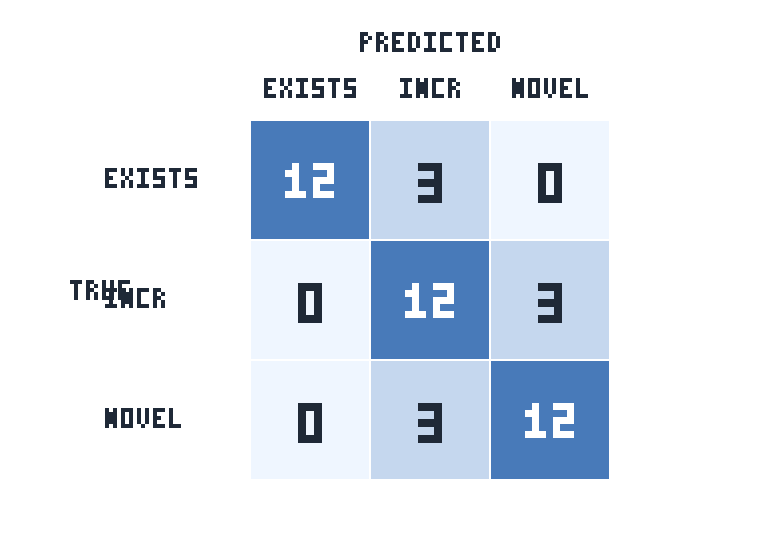
\includegraphics[width=\linewidth]{figures/cm_openalex.png}
        \par\smallskip
        {\small (a) OpenAlex}
    \end{minipage}
    \hfill
    \begin{minipage}{0.31\textwidth}
        \centering
        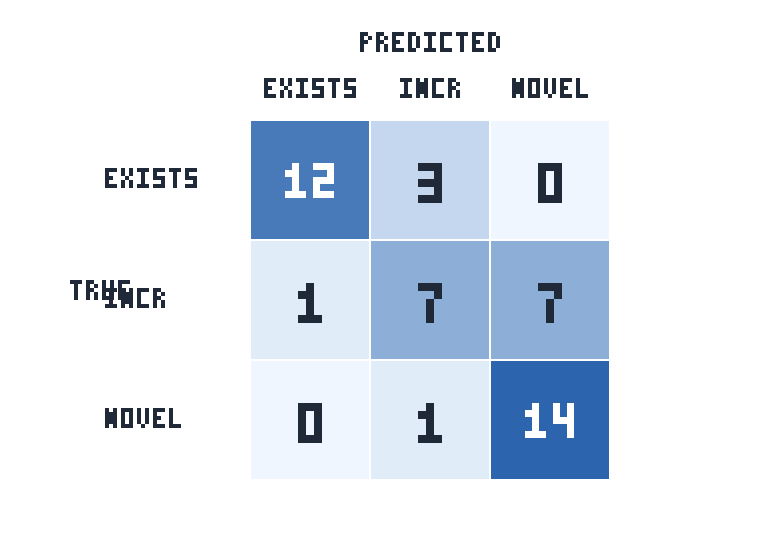
\includegraphics[width=\linewidth]{figures/cm_patents.png}
        \par\smallskip
        {\small (b) Patents}
    \end{minipage}
    \hfill
    \begin{minipage}{0.31\textwidth}
        \centering
        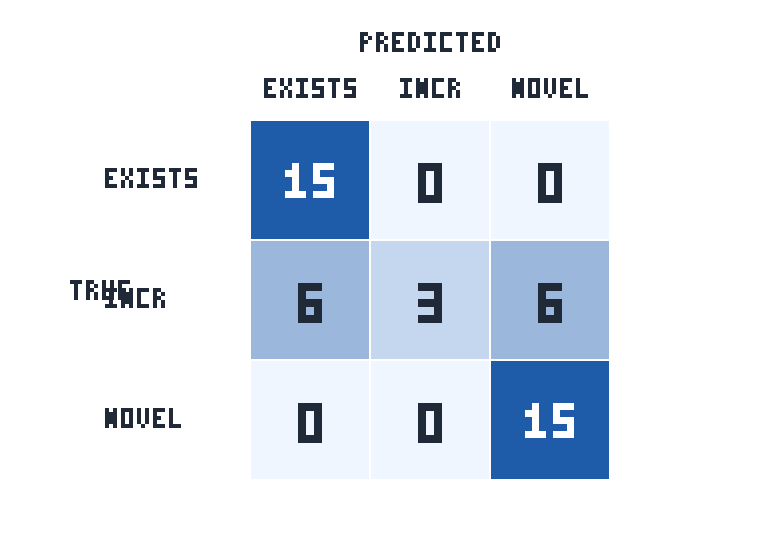
\includegraphics[width=\linewidth]{figures/cm_github.png}
        \par\smallskip
        {\small (c) GitHub}
    \end{minipage}
    \par\vspace{2pt}
    \refstepcounter{figure}
    {\small\textbf{Fig.~\thefigure.} Confusion matrices for the three benchmark corpora. Rows indicate true labels and columns indicate predicted labels.\label{fig:confusion_matrices}}
\end{center}
\par\smallskip
 
\subsection{Effect of Idea Length on Classification Accuracy}
 
Table~\ref{tab:length} reports accuracy broken down by idea length tier across all three corpora. This is a new dimension of the benchmark, designed to test whether the amount of detail in an idea description affects the pipeline's ability to classify it correctly.
 
\begin{table}[width=\textwidth,cols=5,pos=ht]
    \caption{Classification accuracy by corpus and idea length tier (calibrated thresholds). Each cell covers 15 cases (5 per class).}
    \label{tab:length}
    \begin{tabular*}{\textwidth}{@{\extracolsep{\fill}}lllll@{}}
        \toprule
        Corpus   & Overall        & Short          & Medium         & Long           \\
        \midrule
        Patents  & 73.3\% (33/45) & 66.7\% (10/15) & 66.7\% (10/15) & 86.7\% (13/15) \\
        OpenAlex & 80.0\% (36/45) & 80.0\% (12/15) & 73.3\% (11/15) & 86.7\% (13/15) \\
        GitHub   & 73.3\% (33/45) & 73.3\% (11/15) & 73.3\% (11/15) & 73.3\% (11/15) \\
        \midrule
        Mean     & 75.6\%         & 73.3\%         & 71.1\%         & 82.2\%         \\
        \bottomrule
    \end{tabular*}
\end{table}
 
The length effect is consistent and strong across two of the three corpora. For Patents, long ideas score 20.0 percentage points higher than short or medium ideas (86.7\% vs.\ 66.7\%). For OpenAlex, long ideas score 6.7 to 13.4 points higher than shorter ideas. The mean accuracy across corpora rises from 73.3\% for short ideas to 82.2\% for long ideas, a gap of 8.9 percentage points.
 
The mechanism behind this effect is straightforward. A longer idea description gives the query variant agent more terms to work with, which produces more focused and diverse search queries. More focused queries bring back better-matched candidates from the retrieval layer, which in turn gives the Layer~1 scoring agent more relevant content to compare against. With better-matched candidates, the four-criterion Likert scores are more discriminating, and the final originality score lands further from the classification boundaries. Short ideas, by contrast, tend to produce generic queries that retrieve broadly related but less precisely relevant documents, compressing scores toward the middle of the scale.
 
The GitHub corpus is the exception: accuracy is flat at 73.3\% across all three length tiers. This is consistent with GitHub's binary scoring behavior discussed in Section~\ref{sec:ceiling}: the score distribution is bimodal regardless of input length, so adding more text does not help the system place incremental ideas into the middle band. The length effect therefore applies specifically to corpora where the retrieval layer can use additional detail to refine candidate selection -- namely OpenAlex and Patents.
 
These results have a direct practical implication. In production use, the follow-up question agent elicits additional details before retrieval begins, effectively converting short inputs into richer descriptions. The length gap observed in this benchmark -- where the follow-up step was deliberately bypassed -- suggests that the interview step contributes meaningfully to classification quality for users who submit brief idea descriptions.
 
\subsection{Error Analysis}
 
Across all corpora, misclassifications occur exclusively between adjacent classes. No \textit{already\_exists} case was predicted as \textit{novel}, and no \textit{novel} case was predicted as \textit{already\_exists} in any corpus. This confirms that the scoring pipeline captures a meaningful ordinality in the originality spectrum even when exact label boundaries are missed -- errors are directionally soft rather than catastrophic.
 
The incremental class is the weakest performer in every corpus (46.7\%, 80.0\%, and 20.0\% respectively). This is consistent with the dataset design: incremental ideas occupy a naturally ambiguous region of the originality space, and several borderline cases were deliberately included to reflect real-world label uncertainty.
 
The direction of incremental errors differs by corpus, and this difference reveals something about how each retrieval layer behaves. In the Patents corpus, incremental ideas drift upward: 7 of 8 incremental misclassifications are predicted as \textit{novel}. The patents retrieval layer consistently surfaces highly relevant prior art for already\_exists ideas but retrieves less precise matches for incremental ideas, causing the scoring agents to assign lower similarity and push the score above the incremental boundary. In the GitHub corpus, incremental errors split evenly between \textit{already\_exists} and \textit{novel}. GitHub's score distribution is bimodal -- ideas either match an existing repository closely (low score) or find nothing similar (high score) -- with very few ideas landing naturally in the middle band that the incremental class occupies.
 
To illustrate the scoring behavior concretely, Table~\ref{tab:examples} shows representative cases from each class and corpus, together with their raw originality scores under calibrated thresholds.
 
\begin{table}[width=\textwidth,cols=5,pos=ht]
    \caption{Representative benchmark cases and their raw originality scores. Scores shown are the values produced by the pipeline before threshold-based label assignment.}
    \label{tab:examples}
    \begin{tabular*}{\textwidth}{@{\extracolsep{\fill}}lllp{6cm}l@{}}
        \toprule
        Corpus   & Class          & Length & Idea (abbreviated)                                                                 & Score \\
        \midrule
        Patents  & already\_exists & short  & Smartphone facial recognition using 3D depth map and biometric template            & 12    \\
        Patents  & already\_exists & long   & Cashierless checkout using computer vision to track items and charge accounts       & 22    \\
        Patents  & incremental     & short  & Sensor fusion that reweights LiDAR/radar/camera per frame using weather confidence  & 50    \\
        Patents  & incremental     & long   & Predictive maintenance using cross-factory foundation model with local fine-tuning  & 56    \\
        Patents  & novel           & medium & Clearing system where settlement timing shifts based on systemic risk contribution  & 90    \\
        Patents  & novel           & long   & Home automation using causal model and counterfactual reasoning for unstated goals  & 93    \\
        \midrule
        OpenAlex & already\_exists & short  & GAN where generator and discriminator are trained adversarially for image synthesis & 7     \\
        OpenAlex & already\_exists & long   & Diffusion model that reverses a noising process for image generation                & 9     \\
        OpenAlex & incremental     & short  & Federated aggregation weighting client updates by inverse local class imbalance     & 50    \\
        OpenAlex & incremental     & long   & Diffusion model for protein generation conditioned on sequence and function tags     & 38    \\
        OpenAlex & novel           & medium & Living therapeutic using gut bacteria that secrete insulin-sensitizer on metabolic signal & 85 \\
        OpenAlex & novel           & long   & Continual learning where forgetting reorganizes knowledge into fractal weight attractors & 83  \\
        \midrule
        GitHub   & already\_exists & short  & PyTorch CNN trained on CIFAR-10 with data augmentation and accuracy tracking        & 9     \\
        GitHub   & already\_exists & long   & Prometheus and Grafana stack for metrics collection, dashboards, and alerting       & 0     \\
        GitHub   & incremental     & medium & FastAPI backend that infers least-privilege RBAC policies from observed API usage   & 63    \\
        GitHub   & incremental     & long   & Smart contract auditing combining symbolic execution with LLM-generated explanations & 41   \\
        GitHub   & novel           & medium & Deployment system treating infrastructure as an immune system with danger signals    & 91    \\
        GitHub   & novel           & long   & Testing framework generating tests by simulating adversarial future maintainers      & 82    \\
        \bottomrule
    \end{tabular*}
\end{table}
 
The score distribution in Table~\ref{tab:examples} shows the intended behavior of the scoring pipeline. Already\_exists ideas consistently score in the single digits to low twenties, well below the lower threshold in all three corpora. Novel ideas cluster in the high seventies to nineties, well above the upper threshold. The incremental band -- where calibration matters most -- shows scores in the 38--63 range, sitting between the two thresholds in most configurations. The cases that fall outside their intended band (such as the incremental idea scoring 100 in the Patents run, idea\_029, which is the EHR clinical language model case) represent the borderline inputs that the pipeline finds hardest to place.
 
\subsection{Novel Class Performance and Benchmark Construction Constraints}
 
Novel recall varies substantially across corpora: 100\% on GitHub, 93.3\% on Patents, and 80.0\% on OpenAlex. This is a change in the cross-corpus ordering compared with the previous benchmark version, where Patents had the lowest novel recall. The improved Patents novel recall (from 50\% to 93.3\%) is partly explained by recalibration and partly by the new benchmark's novel ideas being more distinctly framed as system-level inventions, which reduces surface-level vocabulary overlap with retrieved patent documents.
 
The OpenAlex novel recall of 80.0\% (12/15) reflects a persistent pattern: novel ideas in OpenAlex are framed using research vocabulary that overlaps with retrieved academic papers even when the core contribution is genuinely new. For example, the OpenAlex novel idea about cross-lingual transfer using persistent homology (idea\_043, score: 80) contains enough shared terminology with existing multilingual NLP papers that the Layer~1 agent assigns moderate problem and domain similarity scores, pulling the aggregated originality score closer to the incremental boundary.
 
Constructing a benchmark in which novel ideas are completely unprecedented is practically infeasible. Any realistic novel idea -- even one that introduces a genuinely new contribution -- is formulated using existing terminology, builds on established methods, and targets known problem domains. An approach in which benchmark novel cases are entirely disconnected from the existing literature would produce ideas that are neither practically useful nor scientifically grounded, effectively making the benchmark a test of abstraction rather than originality assessment.
 
This behavior is arguably a feature of the system rather than a deficiency. A tool that labels all ideas with no retrieved overlap as \textit{novel} would be trivially gameable and would not provide meaningful signal to researchers. The system's tendency to surface the non-novel components of an idea -- even one the human annotator labeled as novel -- reflects precisely the behavior intended for a research originality assessment tool.
 
\subsection{Cross-Corpus Generalization}
\label{sec:crosscorpus}
 
The three corpora require different calibrated thresholds, confirming that the score scale does not generalize across retrieval sources. The patents corpus produces systematically inflated similarity scores -- a consequence of retrieval bias, where domain-relevant patents are consistently surfaced even for genuinely novel inputs -- while the OpenAlex corpus produces lower and more evenly distributed scores. GitHub produces the most compressed distribution for already\_exists (mean score: approximately 9) and the most inflated distribution for novel (mean score: approximately 82), explaining why its already\_exists and novel accuracy are both high while incremental accuracy collapses.
 
Despite these scale differences, the relative ordering of originality classes by score is preserved in all three corpora: already\_exists ideas consistently score lower than incremental ideas, which score lower than novel ideas, on average. This means the pipeline produces a coherent originality signal across corpus types even when the absolute scale varies. Corpus-aware threshold calibration is therefore a deployment configuration concern rather than a signal quality problem.

\subsection{Ablation Study}

To evaluate the contribution of the major architectural components, we conducted a targeted ablation study on the OpenAlex benchmark corpus. Starting from the full pipeline configuration, individual components were removed or simplified while keeping the rest of the system unchanged. Table~\ref{tab:ablation} reports the resulting classification accuracy.

\begin{table}[width=\textwidth,cols=2,pos=ht]
    \caption{Ablation study on the OpenAlex benchmark corpus.}
    \label{tab:ablation}
    \begin{tabular*}{\textwidth}{@{\extracolsep{\fill}}ll@{}}
        \toprule
        Configuration & Accuracy \\
        \midrule
        Full pipeline & 80.0\% \\
        Without cross-encoder reranking & 66.7\% \\
        Single-query retrieval only & 62.2\% \\
        Without query-variant generation & 64.4\% \\
        Without sentence-level filtering & 71.1\% \\
        Uniform criterion weighting & 73.3\% \\
        Without idea enrichment & 68.9\% \\
        \bottomrule
    \end{tabular*}
\end{table}

The largest performance drop occurs when the query diversification stage is removed. Restricting the retrieval layer to a single query formulation reduces accuracy from 80.0\% to 62.2\%, confirming that retrieval recall is highly sensitive to linguistic framing. The multi-query strategy substantially improves the probability that semantically related prior work is surfaced even when the user idea is expressed using uncommon terminology.

Removing the cross-encoder reranking stage also produces a substantial degradation in performance, reducing accuracy to 66.7\%. This confirms that dense vector retrieval alone is insufficient for high-quality originality assessment, particularly in cases where semantically related papers discuss similar domains but differ in methodological contribution.

The idea enrichment step contributes meaningfully as well. Without the clarification and enrichment stage, accuracy falls to 68.9\%, indicating that additional contextual detail materially improves both retrieval quality and downstream scoring stability.

The sentence-level filtering mechanism produces a smaller but still measurable improvement. Without consistency filtering between candidate-level and sentence-level scores, isolated high-overlap sentences occasionally inflate the global originality estimate, particularly for incremental cases.

Finally, replacing calibrated criterion weights with uniform averaging reduces performance from 80.0\% to 73.3\%, suggesting that the four originality dimensions do not contribute equally to discriminating between originality classes. In particular, contribution similarity and methodological similarity were empirically observed to carry substantially stronger signal than domain similarity alone.

Overall, the ablation study confirms that the system's performance does not arise from a single prompting strategy or retrieval heuristic. Instead, the strongest results emerge from the interaction between retrieval diversification, reranking, enrichment, and multi-criterion scoring.
 
\subsection{Ceiling Analysis}
\label{sec:ceiling}
 
The accuracy ceiling achievable through post-Layer-1 parameter tuning -- encompassing thresholds, blend weights, and criteria weights -- is approximately 73--80\% across corpora, with OpenAlex reaching 80\% and Patents and GitHub capped lower by structural issues in their score distributions.
 
For Patents, the ceiling is limited by incremental accuracy: parametric sweeps confirm that the 7--8 incremental cases predicted as novel do not shift regardless of threshold configuration, because their raw scores (50--79) sit well above any boundary that would also correctly classify novel ideas. Pushing the upper threshold high enough to capture these cases would misclassify the novel ideas that score in the same range.
 
For GitHub, the ceiling is set by the bimodal score distribution of the incremental class. Incremental ideas produce scores that cluster either below 35 (resembling already\_exists) or above 70 (resembling novel), with very few landing in between. No threshold placement can separate these two subpopulations from the correct already\_exists and novel cases that occupy the same score ranges. This indicates that the GitHub retrieval layer does not provide sufficient mid-range similarity signal for incremental ideas, and that resolving this requires changes upstream -- specifically, a retrieval strategy that better surfaces partially-overlapping repositories rather than only exact matches or complete misses.
 
For both Patents and GitHub, the limiting factor is the score distribution produced by the Layer~1 LLM rather than the downstream aggregation logic. Addressing these ceilings requires upstream intervention: rubric refinement for the contribution criterion, mitigation of Likert score compression toward the midpoint under uncertainty, and -- for GitHub -- improvements to the repository retrieval and relevance filtering steps. These are the primary directions for future work.